\documentclass[12pt,letterpaper]{article}
\usepackage[utf8]{inputenc}
\usepackage[margin=1in]{geometry}

\usepackage{booktabs}
\usepackage{tabularx}
\usepackage{float}
\usepackage{hyperref}
\usepackage{indentfirst}
\usepackage{enumerate}
\usepackage[shortlabels]{enumitem}
\usepackage{xcolor}
\usepackage{graphicx}
\usepackage{float}

\title{System Requirements Specification\\\progname}

\author{\authname}

\date{}

%% Comments

\usepackage{color}

\newif\ifcomments\commentstrue %displays comments
%\newif\ifcomments\commentsfalse %so that comments do not display

\ifcomments
\newcommand{\authornote}[3]{\textcolor{#1}{[#3 ---#2]}}
\newcommand{\todo}[1]{\textcolor{red}{[TODO: #1]}}
\else
\newcommand{\authornote}[3]{}
\newcommand{\todo}[1]{}
\fi

\newcommand{\wss}[1]{\authornote{blue}{SS}{#1}} 
\newcommand{\plt}[1]{\authornote{magenta}{TPLT}{#1}} %For explanation of the template
\newcommand{\an}[1]{\authornote{cyan}{Author}{#1}}

%% Common Parts

\newcommand{\progname}{REVITALIZE} % PUT YOUR PROGRAM NAME HERE
\newcommand{\authname}{Team 13, REVITALIZE
\\ Bill Nguyen
\\ Syed Bokhari
\\ Hasan Kibria
\\ Youssef Dahab
\\ Logan Brown
\\ Mahmoud Anklis} % AUTHOR NAMES                  

\usepackage{hyperref}
    \hypersetup{colorlinks=true, linkcolor=blue, citecolor=blue, filecolor=blue,
                urlcolor=blue, unicode=false}
    \urlstyle{same}
                                


\begin{document}

\maketitle

\begin{table}[hp]
\caption{Revision History} \label{TblRevisionHistory}
\begin{tabularx}{\textwidth}{llX}
\toprule
\textbf{Date} & \textbf{Developer(s)} & \textbf{Change}\\
\midrule
September 29th, 2022 & Youssef Dahab & Project Drivers \\
October 1st, 2022 & Youssef Dahab & Added Goals of the Project \\
October 1st, 2022 & Syed Bokhari & Added Functional Requirements and Use Case Diagram \\
October 2nd, 2022 & Bill Nguyen & Added Non-Functional Requirements and Use Case Diagram \\
October 3rd, 2022 & Syed Bokhari & Added Work Partitioning Tables \\
October 4th, 2022 & Youssef Dahab & Added Open issues and New Problems \\
October 5th, 2022 & Youssef Dahab & Completed Project Issues \\
\bottomrule
\end{tabularx}
\end{table}

\newpage
\tableofcontents
\newpage

\section{Project Drivers}

\subsection{The Purpose of the Project}
Sustaining a healthy lifestyle requires people to keep track of their eating, exercising, and sleeping habits. This can prove to be a daunting and time consuming thing to do especially when most people are very busy with their lives. The purpose of this project to create an all in one health and wellness mobile application that allows users to manage their diet, exercise, and sleep. REVITALIZE is designed to supply users with the means to improve their health by providing them with meal recipe's based on their nutritional preferences, a personalized workouts planner and a sleep tracker. 

\subsection{Scope}
REVITALIZE will allow users to find recipes for meals based on nutritional preferences such as calories per meal, diet selections, allergies to avoid and ingredients included. The user will be able to count their calorie and nutrient intake through the nutrition logger. The workout planner will allow users to choose from an already existing list of workouts or construct their own workout schedule along with weights, sets, and repetitions. The sleep tracker will provide users with information regarding their sleep. There will be a focus on improving user experience throughout the application along with supplying users with accurate data regarding their health.

\subsection{Goals of the Project}
The goal of this project is to make REVITALIZE, for it's stakeholders, the go to, easy to use, quick, and accessible all in one mobile application for effectively and efficiently managing a person's diet, exercise, and sleep to improve their overall health and well being. The goal of making REVITALIZE a mobile application is for it to be easily accessible to users from their phone at any time and place. Users do not have to memorize their health goals or write them down on a piece of paper that they carry with them all the time. The goal of documenting this project is for stakeholders to have a physical system documentation of a functional product that they can refer to when needed. Stakeholders will be able to match the application to the documentation.

\subsection{The Stakeholders}

\subsubsection{Primary Stakeholders}
Adults and teenagers who want to improve and keep track of their overall health and wellness via an easy to use, all in one application.

\subsubsection{Secondary Stakeholders}
Individuals who may not use the application directly for themselves or are not directly involved with the use of the application but have an indirect benefit. For instance, personal trainers can use REVITALIZE to keep track of workouts, sleep, and the overall health of their clients.

\subsubsection{Facilitating Stakeholders}
Team 13 members building the REVITALIZE application along with Dr.Spencer Smith and the 4G06 TAs.

\section{Project Constraints}

\section{Context Diagrams}

\section{Functional Decomposition Diagrams}

\subsubsection{Work Partitioning}
\begin{table}[h!]
\caption{Work Partitioning Events}
\centering
\begin{tabularx}{\columnwidth}{|X|X|X|X|X|}
\hline
\centering\textbf{Event Number} & \centering\textbf{Event Name} & \centering\textbf{Input} & \centering\textbf{Output} & \textbf{Date}\\
\hline
1 & Launch the application login page & Touch & Main Calender Menu & October 17th, 2022\\
\hline
2 & Opening the sign up page & Touch & Login Page & October 17th, 2022\\
\hline
3 & Opening the main calender menu & Touch & Diet Menu, Workout Menu, Rest Menu & October 24th, 2022\\
\hline
4 & Opening the diet menu  & Touch & Food List & November 14th, 2022\\
\hline
5 & Opening the workout menu & Touch & Excercise List & November 14th, 2022\\
\hline
6 & Opening the rest menu & Touch & Sleep log &  November 14th, 2022\\
\hline
\end{tabularx}
\end{table}

\begin{table}[h]
\caption{Work Partitioning Summaries}
\centering
\begin{tabular}{|c|p{10cm}|}
\hline
\textbf{Event Number} & \textbf{Summary} \\
\hline
1 & The user, through the touch input, decides to launch the applicaiton.The application launches with the login page and after successful credentials the main calender menu will be shown. \\
\hline
2 & The user, through the touch input, decides to open the sign up page. After successful credentials the login page will be shown. \\
\hline
3 & The user, through the touch input, decides to enter the main calender menu. The user can use touch input to select either the diet menu, workout menu or the rest menu. \\
\hline
4 & The user, through the touch input, decides to enter the diet menu. The user can use touch input to view the list of logged food for the calender day, add custom meals, add recipes and search recipes. The user can also navigate through the calender for previous date food entries. \\
\hline
5 & The user, through the touch input, decides to enter the workout menu. The user can use touch input to view the list of logged excercises for the calender day, add custom excercises, add preset excercises, and update set and repitition values for each excercise. The user can also navigate through the calender for previous date workout entries. \\
\hline
6 & The user, through the touch input, decides to enter the rest menu. The user can use touch input to alter the sleep data for the current calender date if innacurate. The user can also navigate through the calender for previous date sleep logs. \\
\hline
\end{tabular}
\end{table}



\subsection{Use Case Diagram}
\begin{figure}[H]
\centering
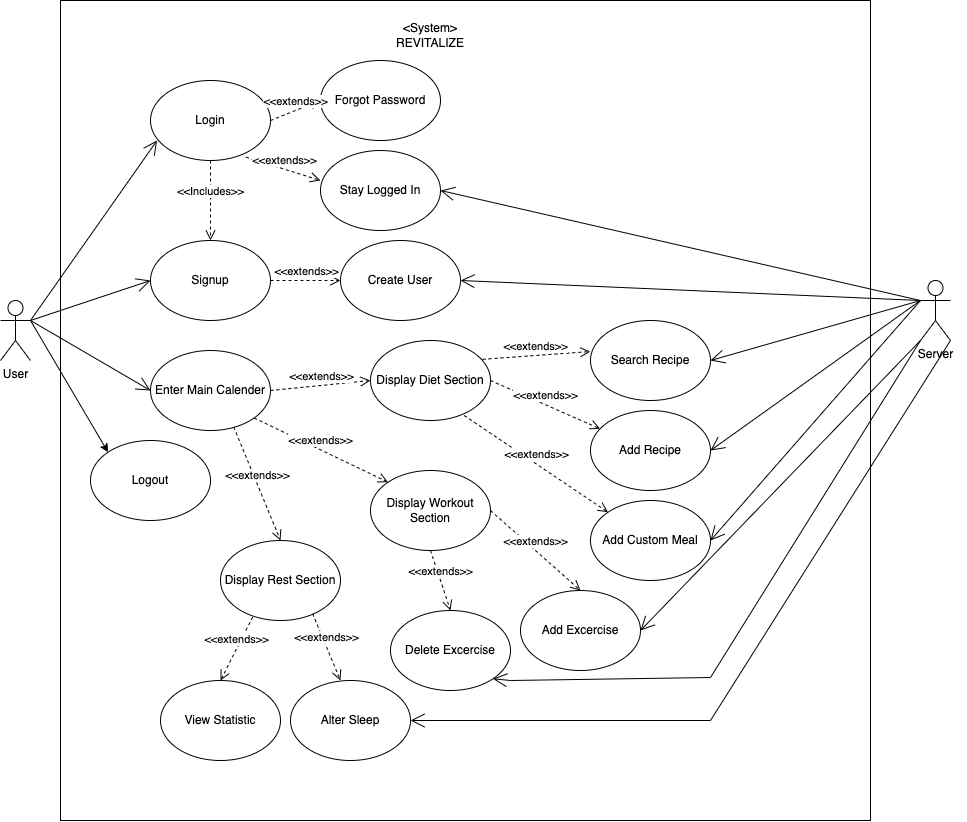
\includegraphics[width=11cm, height=11cm]{4G06SRSUseCaseDiagram.png}
\caption{Use case diagram for REVITALIZE}
\end{figure}

\subsection{Activity Diagram}

\section{Functional Requirements}
\begin{enumerate}[{BE}1.] 
\item The user launches the application
\begin{enumerate}[{FR}1.]
\item  The system must display a login page upon the start of the application.
\item  The login page must display fillable username and password  textboxes
\item  The login page must display a login button
\item  The login page must display a forgot password button
\item  The login page must display a stay logged in checkbox
\item  The system must save prior login information if the stayed logged in checkbox is checked
\item  The login page must display a sign up button that redirects to a signup page
\item  The system msut check the validity of the iput parameters in the login page
\end{enumerate}

\item The user selects the sign up button
\begin{enumerate}[resume*]
\item  The signup page must display fillable username, password, email textboxes
\item  The signup page must display a signup button
\item  The system must check the validity of the input parameters in the signup page
\end{enumerate}

\item The user enters the main page after successful login
\begin{enumerate}[resume*]
\item  The system must display a calender with the current date on successful login
\item  The system must have a previous day and next day button on each page after successful login
\item  The system must display a back button on each user interface after a section is selected
\item  The system must display the sections Diet,Excercise and Rest on the current calender day
\end{enumerate}

\item The user enters the Diet section
\begin{enumerate}[resume*]
\item  The system must prompt the user to height, input dietery, weight,  calorie information on initial launch of Diet section
\item  The system must save initial user height, dietery, wieght, calorie information
\item  The Diet section must initialize with a list of food logged on the current calender day
\item  The Diet section must display an add food button
\item  The Diet section must display a search food button
\item  The search food button must launch a recipe criteria user interface
\item  The recipe criteria user interface must display a list of modifiable criteria and a search button
\item  The recipe search must display correct recipe values based on constraints
\item  The recipe search must display a select recipe and add recipe button
\item  The Diet section must have an add custom meal button
\item  The add custom meal button must have fillable textboxes for recipe information
\item  The previous day and next day button must launch the previous or next calender entry of the user section
\end{enumerate}

\item The user enters the Workout section
\begin{enumerate}[resume*]
\item  The Workout section must initialize with a preset list of excercises on the current calender day
\item  The Workout section must have an add excercise and delete excercise button
\item  The excercises must display an edit excercise button that launches the changeable excercise information when clicked
\item  The Workout section must have an add excercise and delete excercise button
\item  The Workout section must prompt the user to add repititions and sets of each excercise logged in the current calender day
\end{enumerate}

\item The user enters the Rest section
\begin{enumerate}[resume*]
\item  The Rest section must launch with the sleep statistics of the current calender day
\item  The system must allow the user alter innacurate sleep data
\end{enumerate}
\end{enumerate}

\section{Non-functional Requirements}
\noindent Note: followed the volere requirements template

\subsection{Look and Feel Requirements}
\subsubsection{Appearance Requirements}
\begin{enumerate}[{LF}1.] 
\item The application must have a neat and attractive design.\\
{\textbf{Fit Criterion:} A focus group of primary stakeholders such as teenagers and young adults will look at UI/UX design of application and would require an 85\% approval rating.}
\end{enumerate}

\subsubsection{Style Requirements}
\begin{enumerate}[resume*]  
\item The application must use colours that are appealing and contrasting to make it more accessible and non-intrusive.\\
{\textbf{Fit Criterion:} A focus group of primary stakeholders such as teenagers and young adults will test application with a focus on colour and need an 85\% approval rating that the associated colours do not intrude/distract users from overall application.}
\end{enumerate}

\subsection{Usability and Humanity Requirements}
\subsubsection{Ease of Use Requirements}
\begin{enumerate}[{UH}1.] 
\item All aspects and features of mobile application can be used using only one hand/one finger.\\
{\textbf{Fit Criterion:} 95\% of stakeholders with varying size hands/fingers are able to use all aspects of mobile application using one hand/one finger.}
\end{enumerate}
\begin{enumerate}[resume*]  
\item The application home page must be simple so that user can access any feature of application in under 10 seconds\\
{\textbf{Fit Criterion:} 90\% of stakeholders can navigate to any of application features from home page in under 10 seconds. }
\item The application should be easy to use for targeted demographic\\
{\textbf{Fit Criterion:} A focus group of primary stakeholders such as teenagers and young adults with youngest age being 14 will test application and need an 85\% approval rating that application was easy to use. }
\end{enumerate}

\subsubsection{Personalization and Internationalization Requirements}
\noindent NOT AVAILABLE

\subsubsection{Learning Requirements}
\begin{enumerate}[resume*] 
\item Users without any prior experience should be able to use and understand application within 3 iterations of each feature.\\
{\textbf{Fit Criterion:} 85\% of stakeholders can use and understand basic/common aspects of all features within 3 iterations.}
\end{enumerate}

\subsubsection{Understandability and Politeness Requirements}
\begin{enumerate}[resume*] 
\item Associated UI aspects such as buttons, drop-downs, words etc. must be consistent\\
{\textbf{Fit Criterion:} 85\% of stakeholders agree that all UI aspects are simple, consistent and understandable.}
\end{enumerate}

\subsubsection{Accessibility Requirements}
\begin{enumerate}[resume*] 
\item Mobile application should be compatible with android screen readers tool, for potential users with impaired vision.\\
{\textbf{Fit Criterion:} Accessibility tests, will be conducted and 95\% of application UI should be able to be read using an android screen reader tool.}
\end{enumerate}

\subsection{Performance Requirements}
\subsubsection{Speed and Latency Requirements}
\begin{enumerate}[{PE}1.] 
\item All output data of application must take 5 seconds or less to load, based on associated inputs.\\
{\textbf{Fit Criterion:} Developers will run performance tests and ensure all output data loads within 5 seconds or less for 95\% of all API responses and outputs.}
\end{enumerate}

\subsubsection{Safety-Critical Requirements}
\noindent NOT AVAILABLE

\subsubsection{Precision or Accuracy Requirements}
\begin{enumerate}[resume*] 
\item All output data/numbers should be accurate for double precision floating points.\\
{\textbf{Fit Criterion:} Perform associated testing (ex. unit testing) to ensure output is accurate for double precision and passes all test cases. }
\end{enumerate}

\subsubsection{Reliability and Availability Requirements}
\begin{enumerate}[resume*] 
\item Application must have an uptime of 99\%.\\
{\textbf{Fit Criterion:} Description provides all necessary information. }
\end{enumerate}

\subsubsection{Robustness or Fault-Tolerance Requirements}
\noindent NOT AVAILABLE

\subsubsection{Capacity Requirements}
\begin{enumerate}[resume*] 
\item Application can be used by a large amounts of users simultaneously.\\
{\textbf{Fit Criterion:} Application can withstand the usage of at least 50+ users without performance being affected. }
\item Application can store/save large amount of data.\\
{\textbf{Fit Criterion:} Application can store/save 1 million+ of data points for all users. }
\end{enumerate}

\section{Project Issues}

\subsection{Open Issues}
The REVITALIZE team members have not completed their investigation of how to make mobile applications compatible with screen reader tools to make REVITALIZE accessible to users with impaired vision.\\

Moreover, the level of difficulty of maintaining and scaling this project is an open issue as it is highly dependent on the implementation. The team has not yet completed it's assessment of the projection of users, costs, and allocated budget to make a current decision on the maintainability and scalability of the project.\\

Another open issue is regarding the way capacity testing will be conducted:
\begin{itemize}
\item The team has yet to determine how it will find and group a large pool of people simultaneously, ideally 50 or more, to test the application's performance before launch.
\item Determining how to gather large masses user data points, ideally 1 million+, to test the application's storage capacity and performance.
\end{itemize}

\subsection{Off-the-Shelf Solutions}


\subsection{New Problems}
Potential new problems that the REVITALIZE team can encounter include:
\begin{itemize}
\item API failures
\item Server connection errors
\item Copy right issues
\end{itemize}
API failures can occur as a result of connectivity issues, a connection breakdown to the URL, or if it's overloaded with requests from the REVITALIZE application. It is possible to encounter copyright issues when using images from the internet to add visuals to the application. This may or may not complicate the graphical user interface design process. A server connection error is less common but may occur due to a network connection error or if the server is offline.

\subsection{Tasks}
Tasks are scheduled and delegated as per the project \href{https://github.com/BillNguyen1999/REVITALIZE/blob/main/projectschedule/REVITALIZE.pdf}{\color{blue}Gantt Chart}. It will be updated throughout the project to include required tasks and their completion status.

\subsection{Migration to the New Product}
NA

\subsection{Risks}
\begin{itemize}
\item Risk 1: Project may be too complex to complete in eight months because it makes use of multiple built-in and external libraries, other frameworks and application programming interfaces
\begin{itemize}
\item Probability of risk becoming a problem: Medium
\item Contingency plan: Change project scope to meet the minimum number of goals and requirements set by the team to deliver the project
\end{itemize}
\item Risk 2: What if primary stakeholders are not too excited about using the REVITALIZE application after it's launched?
\begin{itemize}
\item Probability of risk becoming a problem: Medium
\item Contingency plan: REVITALIZE team members shall speak to primary stakeholders and listen to their feedback to improve the application.
\end{itemize}
\end{itemize}

\subsection{Costs}
The estimated time cost to deliver this project is eight months. This includes gathering requirements, designing, documenting, implementing, and testing. The cost of launching REVITALIZE to the Google Play Store and App Store are 25\$ and 99\$ respectively.[1]

\subsection{User Documentation and Training}
No user documentation is required to use REVITALIZE. Users will be able to download REVITALIZE as a mobile application from either the Google Play Store or App Store. No training is necessary as using REVITALIZE will be intuitive.

\subsection{Waiting Room}
Ideas that are currently in the waiting room that shall be developed, given enough time, include:
\begin{itemize}
\item Personal Trainer Integration
\begin{itemize}
\item A user's personal trainer can set their diet, workout, and sleep schedules. The trainer can also view user's progress and adjust their schedules.
\end{itemize}
\item Sleep Data Predictor
\begin{itemize}
\item A sleep data predictor that takes users sleep data to extrapolate their health conditions and give tips on optimizing their sleep.
\end{itemize}
\end{itemize}

\subsection{Ideas for Solutions}
Possible ideas to make REVITALIZE accessible to all people include designing clear layouts, increasing font sizes, increasing text visibility, using large buttons and controls, and describing user interface elements. Another idea to prevent API failures is to run tests to monitor and track API performance from early development through production.

\section{Reflection Appendix}

\subsection{Knowledge and Skills Needed}

\noindent Bill Nguyen: Skills that the team needs to acquire are end to end development, CI/CD, multiple ways of testing (integration, unit, acceptance tests etc...). This will be needed since project is end to end (front-end, back-end, database etc.), will be using CI/CD to deploy code changes, and will be testing project in multiple ways.\\

\noindent Syed Bokhari: Skills relating to API integration and server communication are needed for the technical development of the application. This is needed because the project depends on the use of multiple APIs for the core functionality of its features. Knowledge of server communication is required due to the nature of application development as the dynamic application information requires constant feedback from the server. 

\subsection{How Knowledge and Skills Will Be Acquired}

\noindent Bill Nguyen: Project will be end to end so will implement code in front-end, back-end etc. and will be integrating all components to make it an end to end project. Will use CI/CD in project to integrate and deploy code, so will add necessary steps in yaml file to make and update CI/CD process. Will research and implement unit, integration, acceptance tests etc. to learn more about multiple types of tests. \\

\noindent Syed Bokhari: The knowledge relating to API integration will be acquired through reading API specific documentation and creating test API applications to test the correct functionality of each API in use. The server communication will be learned through research and development of the project.



\newpage 

\section{References}
[1] \href{https://www.appypie.com/faqs/how-much-does-it-cost-to-publish-an-app-on-the-app-store}{\color{blue}How much does it cost to publish an app on the app store?}

\end{document}